%=============================================================
% tmfeo3_chi_selection_rules.tex
% Chi coupling selection rules in TmFeO3 Gamma_2 phase
% Companion to util/analyze_chi_selection_rules.py and
% src/apps/diag_tmfeo3_qafm_e12_xpeak.cpp
%=============================================================
\documentclass[11pt,a4paper]{article}
\usepackage[margin=2.5cm]{geometry}
\usepackage{amsmath,amssymb,bm,mathtools,booktabs,array,tabularx,multirow}
\usepackage{graphicx}
\usepackage{xcolor}
\usepackage{hyperref}
\usepackage{tikz}
\usetikzlibrary{arrows.meta,positioning}
\usepackage{caption}
\usepackage{subcaption}
\usepackage[T1]{fontenc}

\hypersetup{colorlinks=true,linkcolor=blue,citecolor=blue,urlcolor=blue}

% ---- notation shortcuts ----
\newcommand{\sF}{\sigma_F}
\newcommand{\sG}{\sigma_G}
\newcommand{\sA}{\sigma_A}
\newcommand{\sC}{\sigma_C}
\newcommand{\vlam}{\bm{\lambda}}
\newcommand{\vS}{\bm{S}}
\newcommand{\Heff}{\mathcal{H}}
\newcommand{\etaz}{\eta^z}
\newcommand{\etax}{\eta^x}
\newcommand{\etay}{\eta^y}
\newcommand{\diag}{\mathrm{diag}}
\newcommand{\Mz}{M_z^{\mathrm{Tm}}}
\newcommand{\lamt}{\lambda^2}
\newcommand{\lamf}{\lambda^5}
\newcommand{\FeOs}{TmFeO$_3$}
\newcommand{\Gtwo}{\Gamma_2}
\newcommand{\GzGz}{G_z}
\newcommand{\qAFM}{\mathrm{qAFM}}
\newcommand{\EtA}{E_{12}}
\newcommand{\crossP}{(\omega_{\qAFM},\,\omega_{\EtA})}

\definecolor{passgreen}{HTML}{27AE60}
\definecolor{failred}{HTML}{E74C3C}
\definecolor{warnora}{HTML}{E67E22}
\definecolor{lightblue}{HTML}{EAF4FB}
\definecolor{lightgreen}{HTML}{D5F5E3}
\definecolor{lightred}{HTML}{FADBD8}

\title{\textbf{Chi Coupling Selection Rules in TmFeO$_3$ $\Gamma_2$ Phase}\\[4pt]
\large Ground-State Lambda Generation and qAFM Cross-Peak Detectability\\
under $H\parallel c$ (2DCS Geometry)}
\author{}
\date{June 2026}

\begin{document}
\maketitle
\tableofcontents
\bigskip\bigskip

%--------------------------------------------------------------
\section{Overview and main result}
%--------------------------------------------------------------

We analyse all nine $\chi_{2\alpha}$, $\chi_{5\alpha}$, $\chi_{7\alpha}$
coupling channels ($\alpha \in \{x,y,z\}$) of the mixed Fe--Tm Hamiltonian
in \FeOs{} in its $\Gtwo$ ($G_z$, $F_x$) magnetic phase.  The central
question is whether the cross-peak at excitation frequency $\omega_{\qAFM}$
and detection frequency $\omega_{\EtA}$ (the Tm $|E_1\rangle\!\to\!|E_2\rangle$
transition) can be nonzero in a $H\parallel c$ 2DCS experiment.

\medskip
\noindent\colorbox{lightred}{%
\parbox{\dimexpr\linewidth-2\fboxsep}{%
\textbf{Result}: The cross-peak $\crossP$ is \emph{doubly forbidden} for
every chi channel by the following two independent Bertaut-vector orthogonality
constraints:
\begin{enumerate}
  \item \textbf{Source failure}: in the $\Gtwo$ phase no chi channel produces
    $\sC$-pattern $\lamt$.  Every channel produces either zero or
    $\sF$-pattern $\lamt$.
  \item \textbf{Detector failure}: $H\parallel c$ couples to
    $\Mz = c_2\,(\sC \cdot \vlam^2_{\mathrm{vec}})$.
    Since $\sC\cdot\sF = 0$, the signal vanishes even when $\lamt$ is large.
\end{enumerate}
}}

\medskip
The proof rests on two exact algebraic identities of the Bertaut sigma vectors
(Sec.~\ref{sec:sigma}) together with the bond connectivity and local-frame
conventions of \texttt{unitcell\_builders.cpp} (Sec.~\ref{sec:frames}).
Numerical verification is provided by the diagnostic executable
\texttt{diag\_tmfeo3\_qafm\_e12\_xpeak} (Sec.~\ref{sec:numeric}).

%--------------------------------------------------------------
\section{Sigma vectors and Bertaut orthogonality}
\label{sec:sigma}
%--------------------------------------------------------------

The four Pbnm sublattice-staggering patterns are defined as four-component
vectors in the order $(\mu=0,1,2,3)$:
\begin{equation}
  \sF = (+,+,+,+), \quad
  \sG = (+,-,+,-), \quad
  \sA = (+,+,-,-), \quad
  \sC = (+,-,-,+).
\end{equation}
They form an orthogonal set under the sublattice inner product
$\sigma_P \cdot \sigma_Q = \sum_{\mu=0}^{3} \sigma_P[\mu]\,\sigma_Q[\mu]$:
\begin{equation}
  \sigma_P \cdot \sigma_Q = 4\,\delta_{PQ},
  \quad P,Q \in \{F,G,A,C\}.
  \label{eq:orth}
\end{equation}
The component-wise product rule (Hadamard product) closes within the set:
\begin{equation}
  \sG \circ \sG = \sF, \quad
  \sA \circ \sG = \sC, \quad
  \sC \circ \sG = \sA, \quad
  \sA \circ \sA = \sF, \quad
  \sC \circ \sC = \sF, \quad \ldots
  \label{eq:had}
\end{equation}

%--------------------------------------------------------------
\section{Fe and Tm local frames}
\label{sec:frames}
%--------------------------------------------------------------

\subsection{Fe sublattice frames}

The four Fe sublattices sit at Wyckoff 4b positions.  Their local frames
(stored as \texttt{R\_fe\_frames} in \texttt{unitcell\_builders.cpp}) are
diagonal:
\begin{equation}
  R^{(k)}_{\mathrm{Fe}} = \diag\bigl(\eta^x_k,\,\eta^y_k,\,\eta^z_k\bigr),
  \quad k = 0,1,2,3.
\end{equation}
The diagonal entries and their sublattice patterns are:
\begin{center}
\begin{tabular}{cllll}
\toprule
 & Fe$_0$ ($E$) & Fe$_1$ ($C_{2x}$) & Fe$_2$ ($C_{2z}$) & Fe$_3$ ($C_{2y}$) \\
\midrule
$\eta^x$ & $+1$ & $+1$ & $-1$ & $-1$ \\
$\eta^y$ & $+1$ & $-1$ & $-1$ & $+1$ \\
$\eta^z$ & $+1$ & $-1$ & $+1$ & $-1$ \\
\midrule
pattern & \multicolumn{2}{l}{$\etax_{\mathrm{Fe}} = \sA$} & \multicolumn{2}{l}{} \\
        & \multicolumn{2}{l}{$\etay_{\mathrm{Fe}} = \sC$} & \multicolumn{2}{l}{} \\
        & \multicolumn{2}{l}{$\etaz_{\mathrm{Fe}} = \sG$} & \multicolumn{2}{l}{} \\
\bottomrule
\end{tabular}
\end{center}

The Fe spin is stored in the global lab frame, so the local component along
axis $\alpha$ is $S^\alpha_{\mathrm{loc},k} = R^{(k)}_{\alpha\alpha}\,S^\alpha_k
= \eta^\alpha_k\,S^\alpha_k$.

\subsection{Tm sublattice frames}

The four Tm sublattices sit at Wyckoff 4c positions.  Their local frames
(from \texttt{tmfeo3\_tm\_local\_frames\_xyz()}) are also diagonal:
\begin{center}
\begin{tabular}{cllll}
\toprule
 & Tm$_0$ & Tm$_1$ & Tm$_2$ & Tm$_3$ \\
\midrule
$\eta^x$ & $+1$ & $+1$ & $-1$ & $-1$ \\
$\eta^y$ & $+1$ & $-1$ & $+1$ & $-1$ \\
$\eta^z$ & $+1$ & $-1$ & $-1$ & $+1$ \\
\midrule
pattern & \multicolumn{2}{l}{$\etax_{\mathrm{Tm}} = \sA$} & \multicolumn{2}{l}{} \\
        & \multicolumn{2}{l}{$\etay_{\mathrm{Tm}} = \sG$} & \multicolumn{2}{l}{} \\
        & \multicolumn{2}{l}{$\etaz_{\mathrm{Tm}} = \sC$} & \multicolumn{2}{l}{} \\
\bottomrule
\end{tabular}
\end{center}

The physical Tm magnetic moment along the global $z$-axis is
\begin{equation}
  J^z_{j,\mathrm{glob}} = \etaz_{\mathrm{Tm},j}\,J^z_{j,\mathrm{loc}}
                        = \sC[j]\,c_2\,\lamt_j,
  \label{eq:Jzglob}
\end{equation}
where $c_2 = \langle E_1|J^z|E_2\rangle_{\mathrm{loc}}$ is the local Tm CEF
matrix element, and $\lamt$ is the imaginary part of the $|E_1\rangle$--$|E_2\rangle$
coherence (second Gell-Mann component).

\subsection{Bond connectivity: each Tm sees all four Fe}

From \texttt{fe\_tm\_w\_bond\_pairs()} there are 4 orbits $\times$ 2 bonds (even/odd)
= 16 bond pairs in the unit cell.  A key property is:
\begin{equation}
  \text{Each Tm sublattice $j$ has exactly one bond per orbit,
  connecting it to each of the four Fe sublattices.}
\end{equation}
Consequently, summing the chi coupling over all bonds to Tm$_j$ is equivalent
to the inner product over all Fe sublattices:
\begin{equation}
  H^\alpha_{\chi,j}[\lamt]
    = \chi_{2\alpha}\sum_{k=0}^{3} \eta^\alpha_{\mathrm{Fe},k}\,S^\alpha_{\mathrm{Fe},k}.
  \label{eq:Hchi_sum}
\end{equation}

Figure~\ref{fig:bonds} shows the 3D crystal structure with all 16 even bonds
coloured by orbit.  Figure~\ref{fig:fe_frames} shows the Fe local frame axes
(arrows) at each sublattice position.

\begin{figure}[h!]
  \centering
  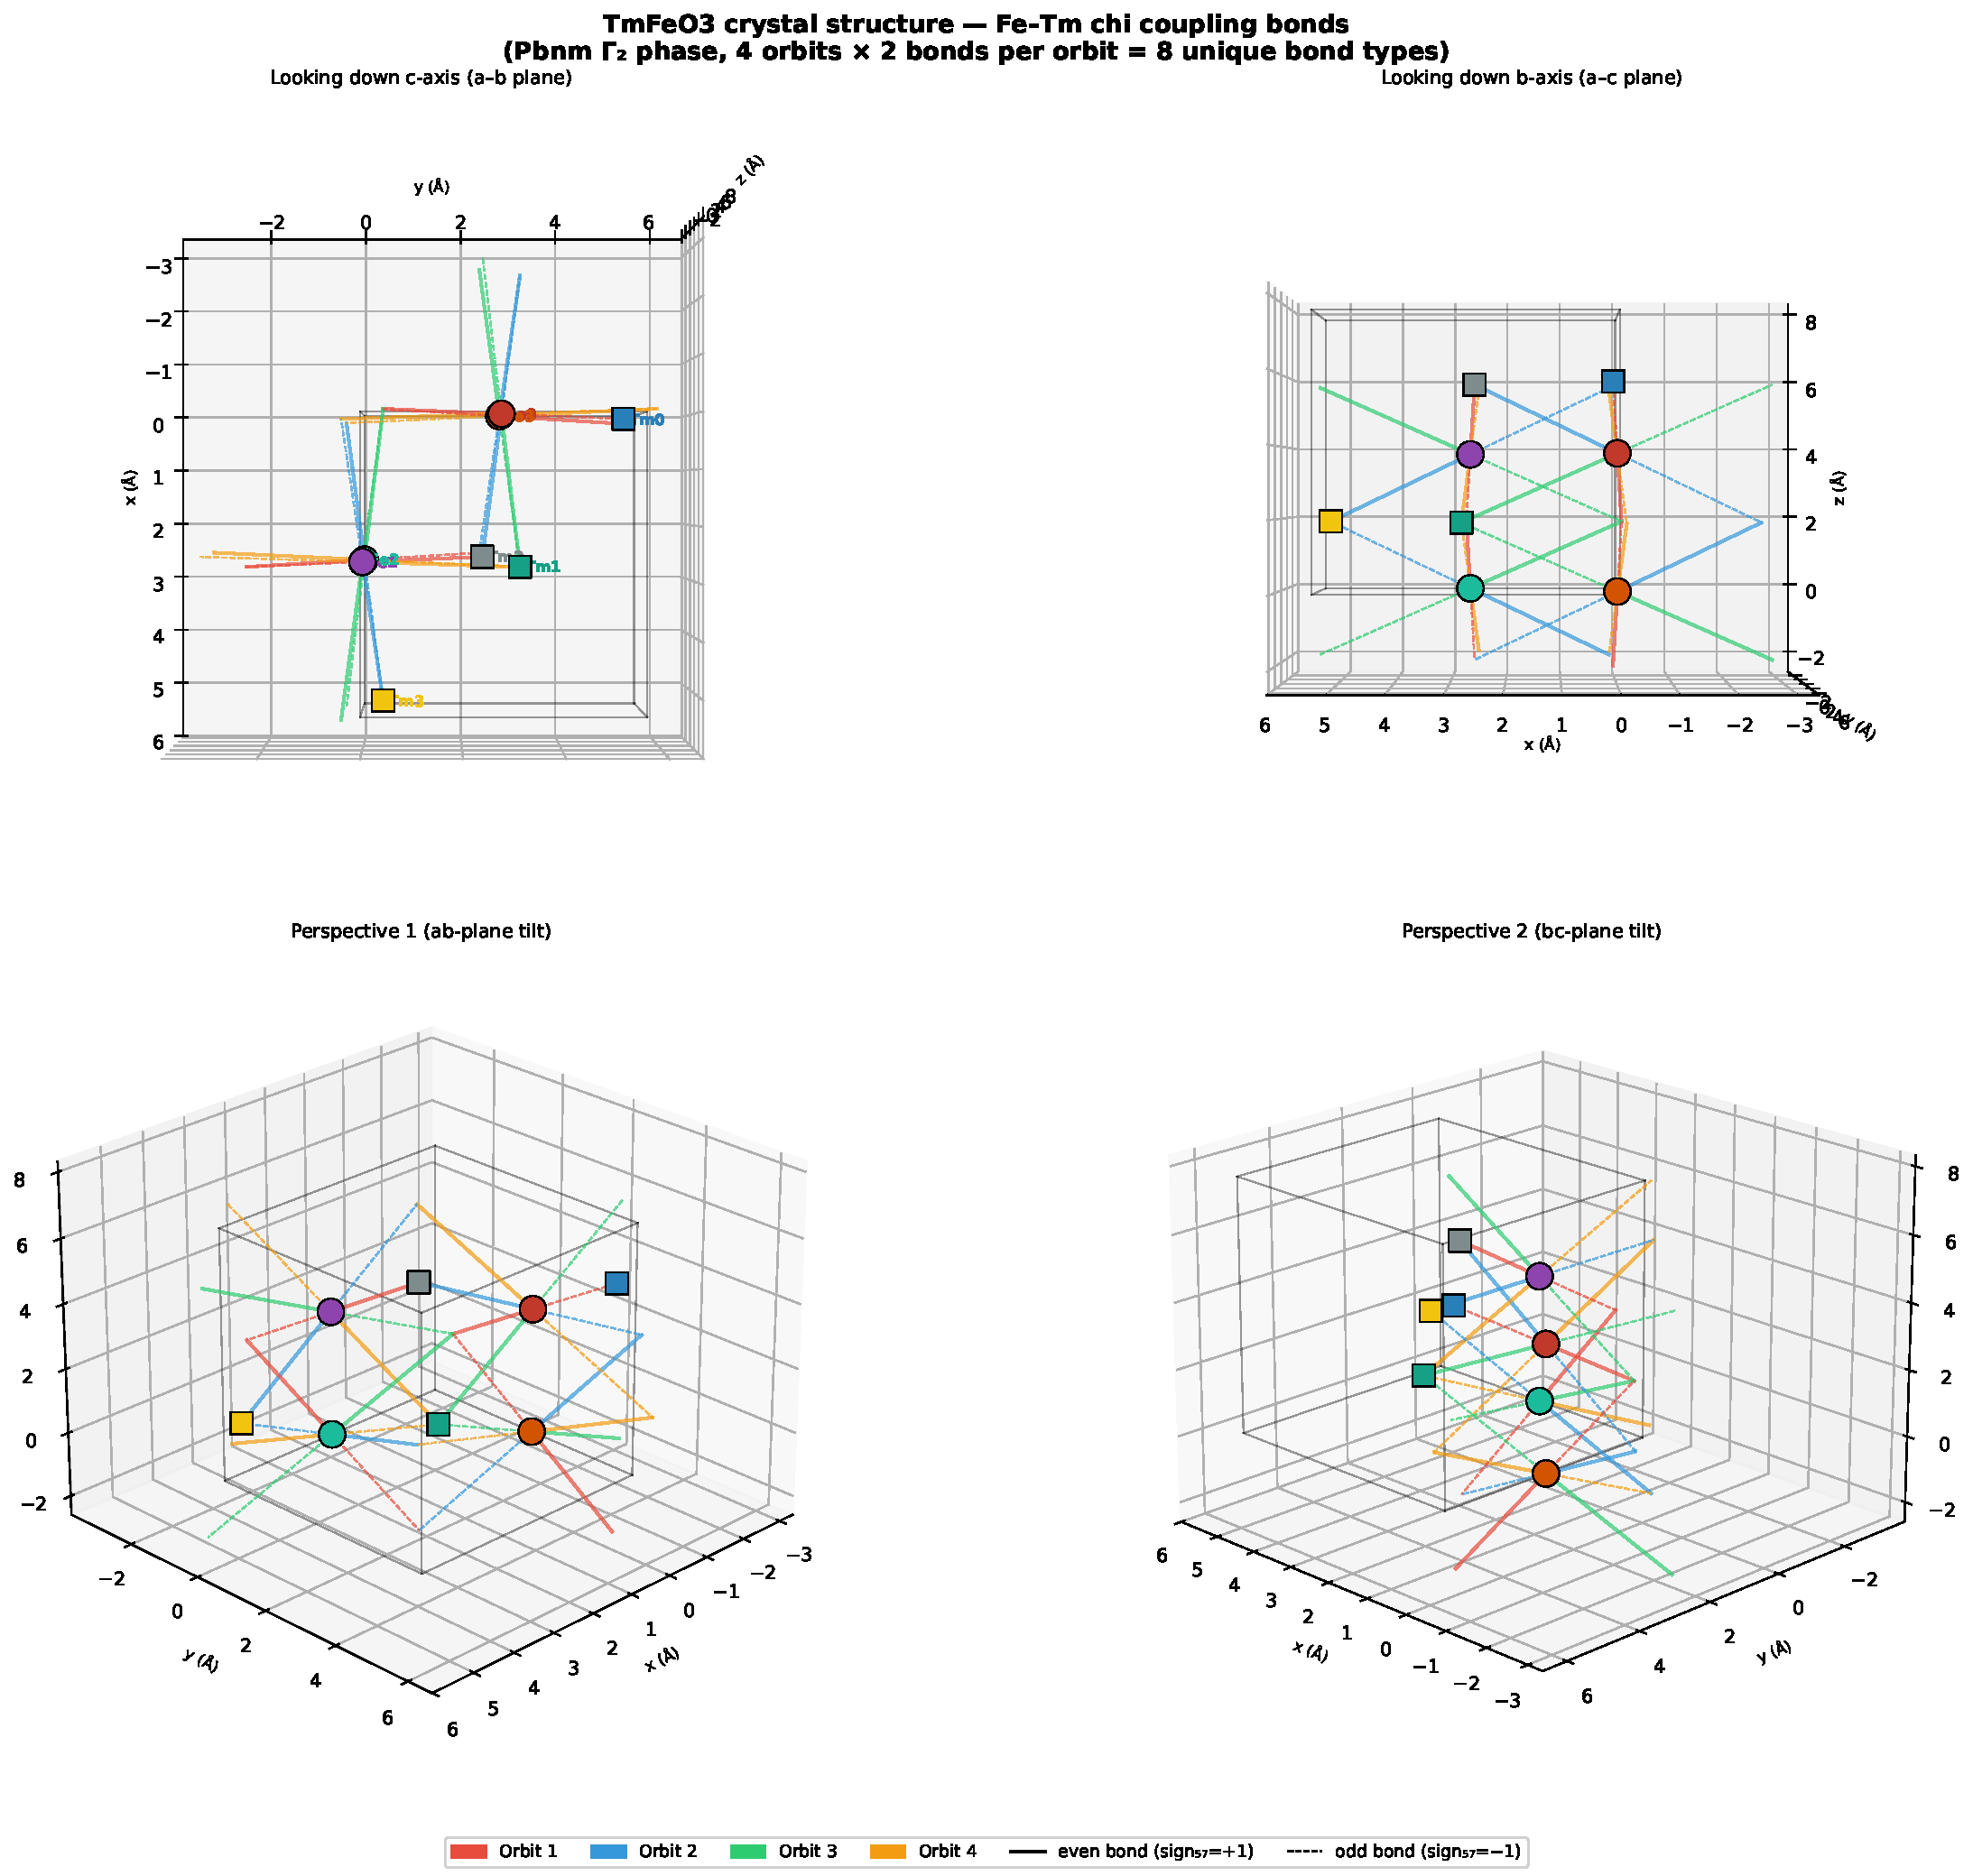
\includegraphics[width=\textwidth]{chi_bonds_3d_structure.pdf}
  \caption{TmFeO$_3$ crystal structure with Fe–Tm chi coupling bonds.  Circles:
    Fe sublattices (red/purple/teal/orange = sub 0/1/2/3).  Squares: Tm sublattices
    (blues/greys/yellow).  Solid lines: even bonds (sign$_{57}=+1$); dashed: odd
    bonds (sign$_{57}=-1$).  Colours: orbit 1 (red), 2 (blue), 3 (green), 4 (orange).
    Each Tm sublattice has exactly one bond per orbit, connecting it to all four
    Fe sublattices.}
  \label{fig:bonds}
\end{figure}

\begin{figure}[h!]
  \centering
  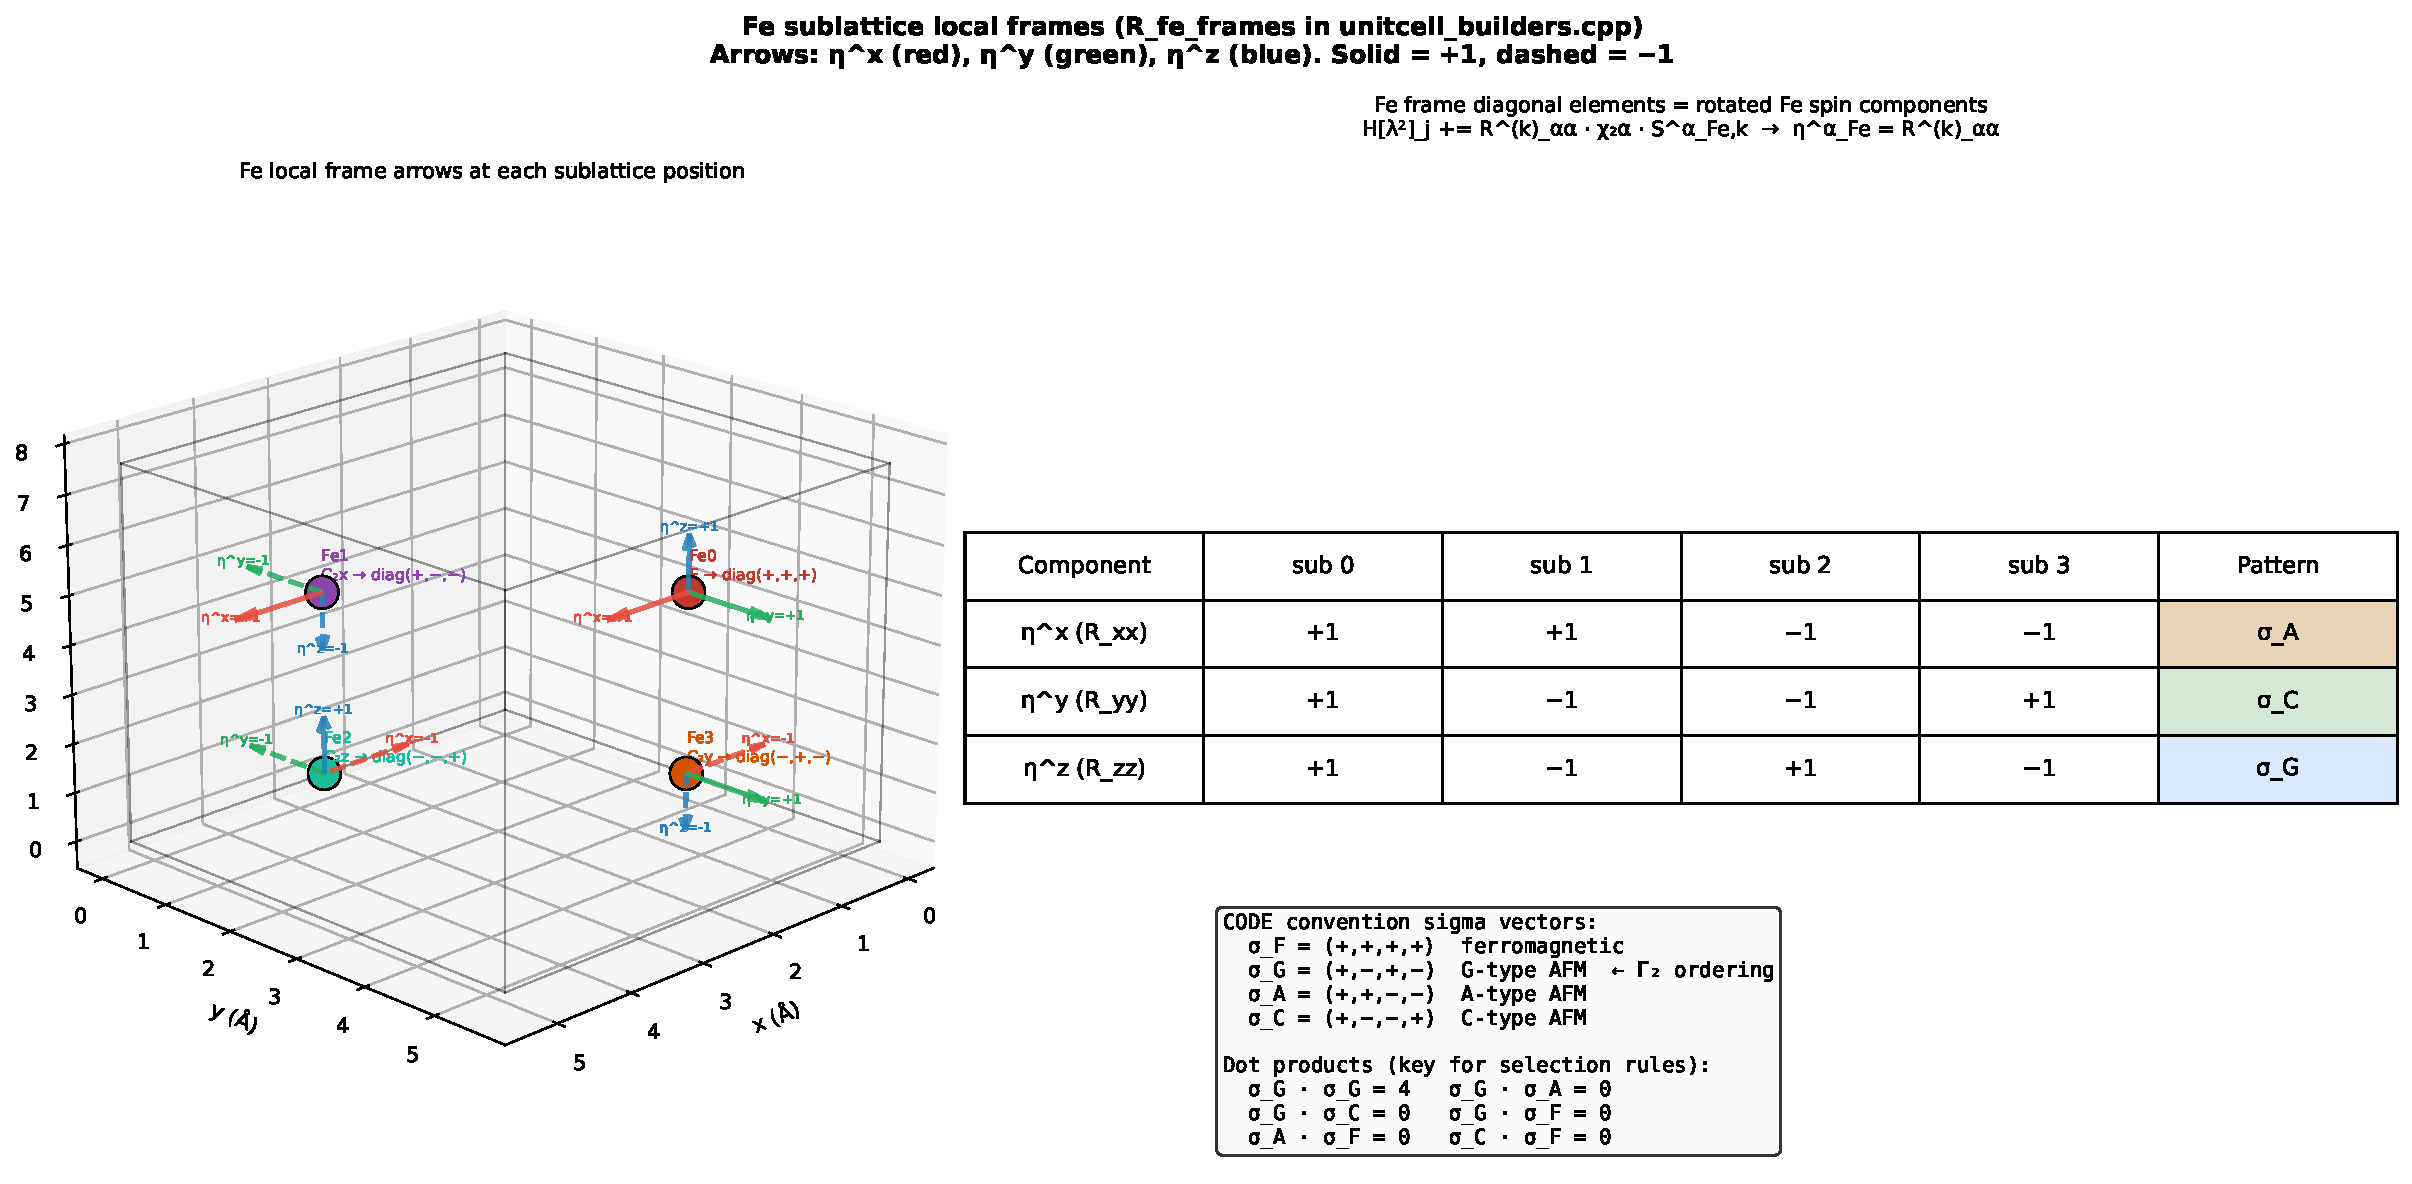
\includegraphics[width=\textwidth]{chi_fe_frames.pdf}
  \caption{\emph{Left}: Fe local frame arrows at each sublattice position.
    Red $=\hat{x}$, green $=\hat{y}$, blue $=\hat{z}$.  Solid arrow: $\eta=+1$;
    dashed: $\eta=-1$.
    \emph{Right}: Summary table of Fe frame diagonal elements and their
    Bertaut patterns.  The right-hand panel also lists the Bertaut inner products
    most relevant for the selection rules.}
  \label{fig:fe_frames}
\end{figure}

\begin{figure}[h!]
  \centering
  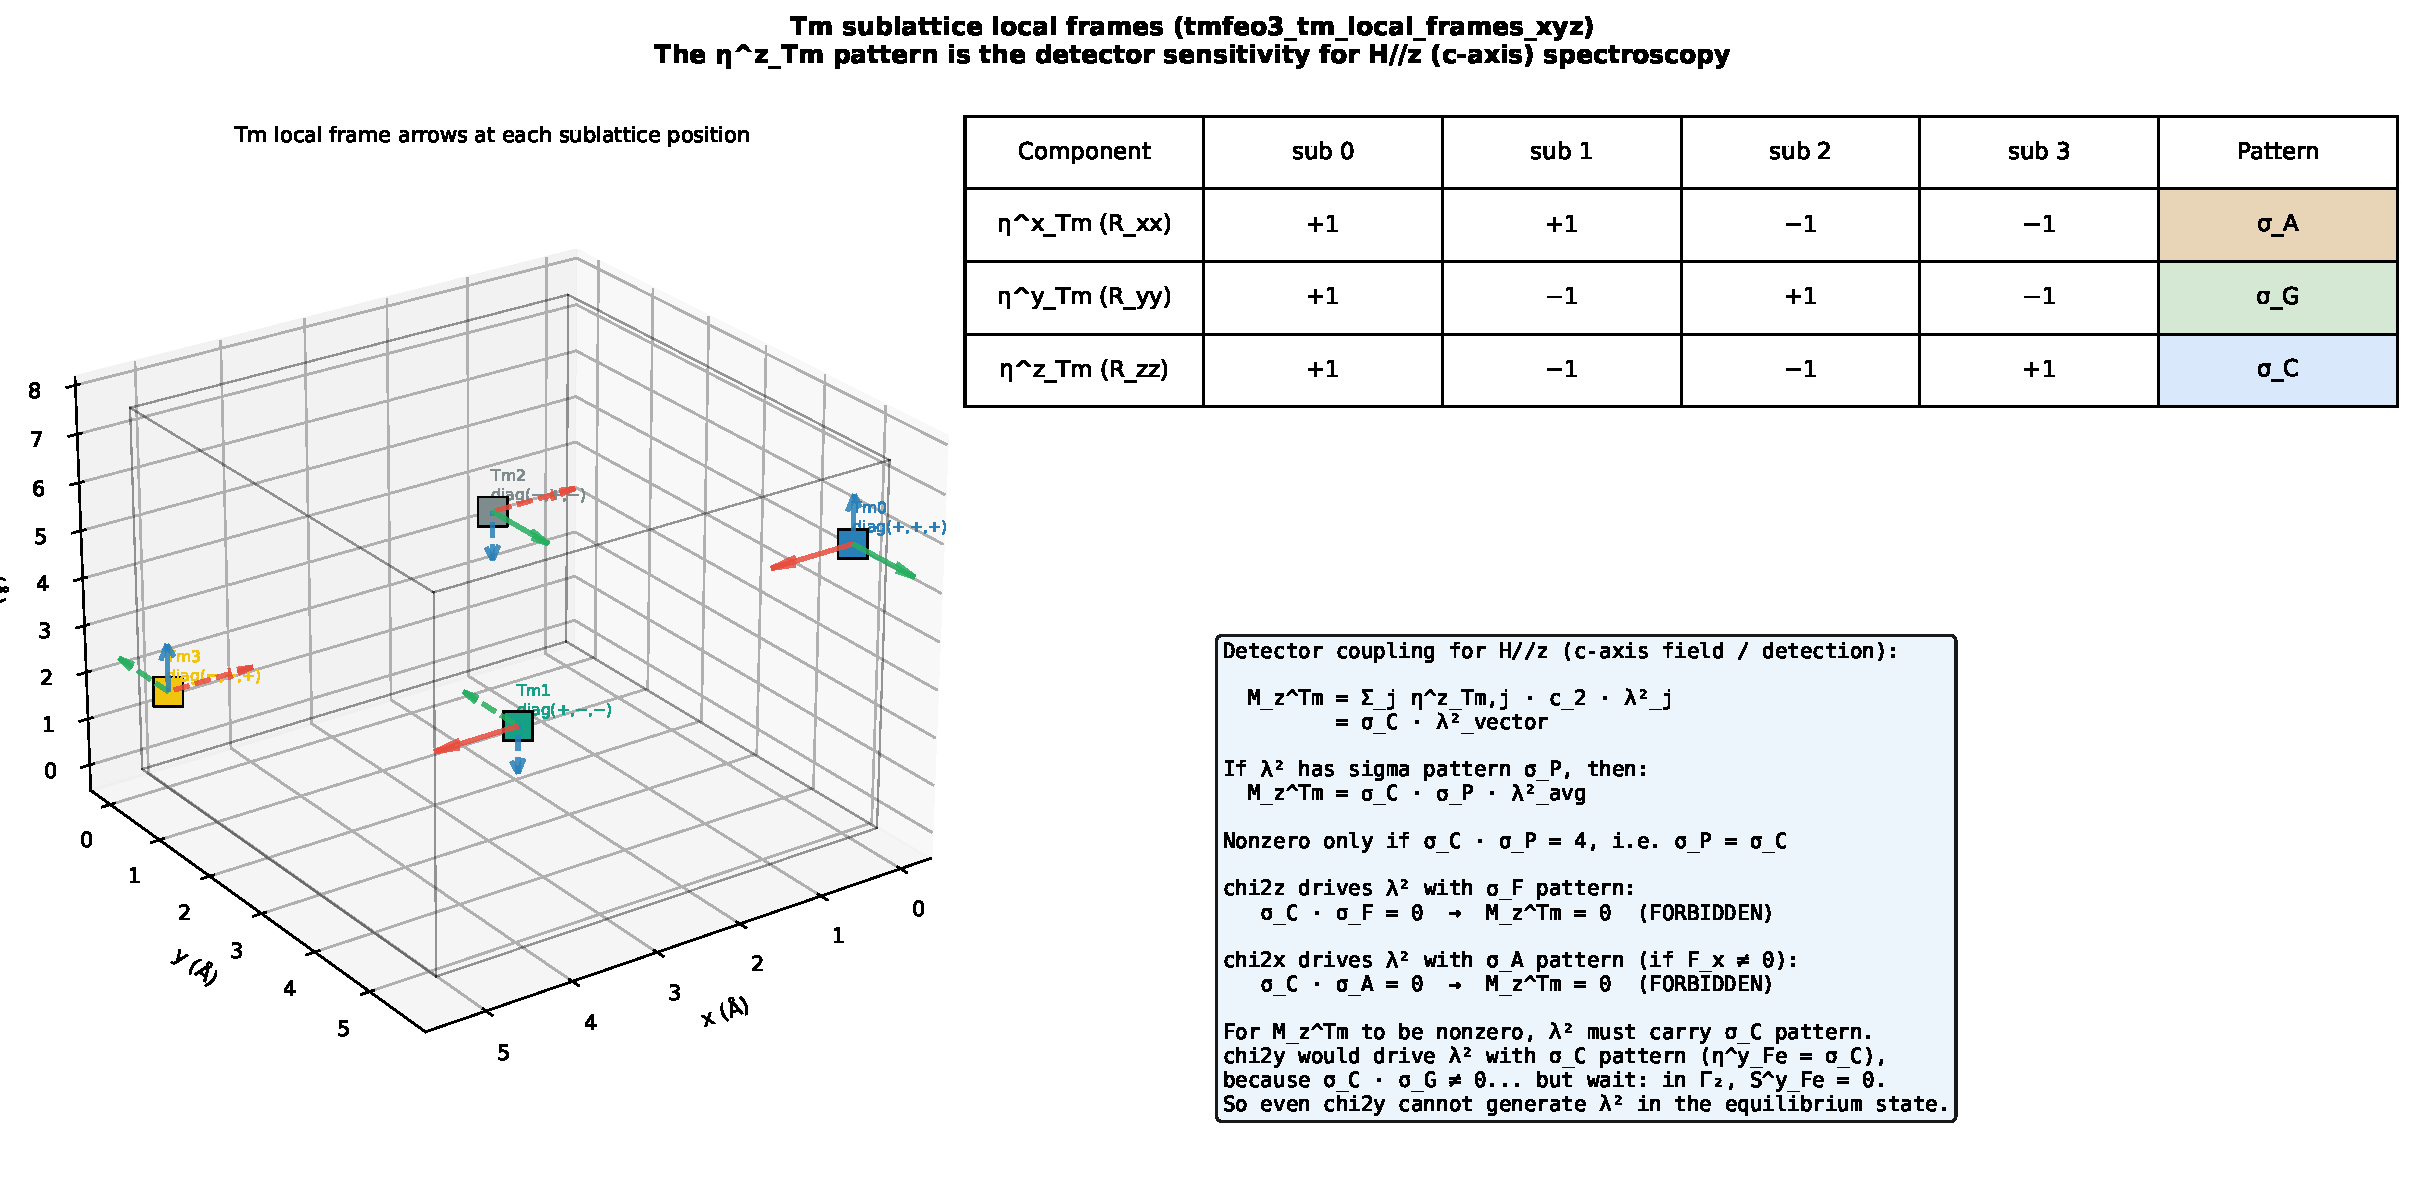
\includegraphics[width=\textwidth]{chi_tm_frames.pdf}
  \caption{\emph{Left}: Tm local frame arrows.
    \emph{Right}: Tm frame patterns and the detector coupling analysis.
    $\etaz_{\mathrm{Tm}} = \sC = (+,-,-,+)$, so $H\parallel c$ detects
    $\Mz = c_2\,(\sC\cdot\vlam^2_{\mathrm{vec}})$.  For this to be nonzero,
    $\lamt$ must carry $\sC$ pattern.}
  \label{fig:tm_frames}
\end{figure}

%--------------------------------------------------------------
\section{Ground-state analysis: which channels activate $\lambda^2$}
\label{sec:gs}
%--------------------------------------------------------------

\subsection{Gamma$_2$ Fe spin background}

In the $\Gtwo$ ($G_z$, $F_x$) magnetic phase:
\begin{equation}
  S^z_{\mathrm{Fe},k} = G_z\,\sG[k], \quad
  S^x_{\mathrm{Fe},k} = F_x\,\sF[k], \quad
  S^y_{\mathrm{Fe},k} = 0,
  \label{eq:G2spins}
\end{equation}
where $G_z \approx 2.5\,\mu_B$ and $F_x \approx 0.014\,\mu_B$
($F_x/G_z \approx 0.006$, set by the DM ratio $D_1/H_E$).

\subsection{Effective field on $\lamt$ from each chi channel}

Substituting \eqref{eq:G2spins} into \eqref{eq:Hchi_sum}:
\begin{align}
  H[\lamt]_j^{\chi_{2z}}
    &= \chi_{2z}\sum_{k}\sG[k]\cdot G_z\sG[k]
     = \chi_{2z}\,G_z\sum_{k}\sG[k]^2
     = 4\chi_{2z}\,G_z.
  \label{eq:H2z}\\[4pt]
  H[\lamt]_j^{\chi_{2x}}
    &= \chi_{2x}\sum_{k}\sA[k]\cdot F_x\sF[k]
     = \chi_{2x}\,F_x\,(\sA\cdot\sF) = 0.
  \label{eq:H2x}\\[4pt]
  H[\lamt]_j^{\chi_{2y}}
    &= \chi_{2y}\sum_{k}\sC[k]\cdot 0 = 0.
  \label{eq:H2y}
\end{align}

Key observations:
\begin{itemize}
  \item Equation~\eqref{eq:H2z}: $\sG[k]^2 = 1$ for each $k$, so the sum
    is $+4$ at \emph{every} Tm sublattice identically.
    The resulting $\lamt_j$ is \textbf{uniform} ($\sF$-pattern).
    Numerical value: $\lamt \approx -0.997\,\sF$ at equilibrium
    (from \texttt{diag\_tmfeo3\_qafm\_e12\_xpeak}).
  \item Equation~\eqref{eq:H2x}: $\sA\cdot\sF = \sum_k(+,+,-,-)(+,+,+,+)= 0$.
    The small $F_x$ canting is invisible to $\chi_{2x}$.
  \item Equation~\eqref{eq:H2y}: $S^y_{\mathrm{Fe}}=0$ in $\Gtwo$, so
    $\chi_{2y}$ is completely inert.
\end{itemize}

\subsection{Chi5 and chi7: exact cancellation by the inversion sign}

For $\chi_{5\alpha}$ (coupling to $\lambda^5$), the bond tensor acquires
a factor $\mathrm{sign}_{57} = \pm1$: the even bond of each orbit pair
carries $+1$, and the odd (inversion-related) bond carries $-1$.  Crucially,
within each orbit pair, \emph{both bonds connect the same Fe sublattice} to
(different) Tm sites.  Therefore the net contribution per Tm site is:
\begin{equation}
  H[\lambda^5]_j \propto (+1)\,\eta^\alpha_{\mathrm{Fe},k}\,S^\alpha_k
                        + (-1)\,\eta^\alpha_{\mathrm{Fe},k}\,S^\alpha_k = 0.
\end{equation}
The cancellation is exact for all Fe spin configurations ($\chi_5$ and
$\chi_7$ are dead at $q=0$ for \emph{any} magnetic order).

%--------------------------------------------------------------
\section{The H$\parallel c$ detector coupling}
\label{sec:detector}
%--------------------------------------------------------------

The Tm contribution to the $z$-magnetisation observable is (from
Eq.~\eqref{eq:Jzglob}):
\begin{equation}
  \boxed{
    \Mz = g_J\mu_B\sum_{j=0}^{3} \sC[j]\,c_2\,\lamt_j
        = g_J\mu_B\,c_2\,(\sC\cdot\vlam^2_{\mathrm{vec}}).
  }
  \label{eq:Mz}
\end{equation}

From the ground-state result (Sec.~\ref{sec:gs}), $\lamt_j \approx
\bar\lambda^2\,\sF[j]$, so:
\begin{equation}
  \Mz = g_J\mu_B\,c_2\,\bar\lambda^2\,(\sC\cdot\sF)
      = g_J\mu_B\,c_2\,\bar\lambda^2\cdot 0 = 0,
\end{equation}
using $\sC\cdot\sF = (+,-,-,+)\cdot(+,+,+,+) = 1-1-1+1=0$.

This is the first selection rule: \textbf{even though $\chi_{2z}$ generates
large $\lamt \approx \pm 1$, the signal $\Mz$ is identically zero because
the $\sF$ pattern of $\lamt$ is orthogonal to the $\sC$ detector pattern.}

\begin{figure}[h!]
  \centering
  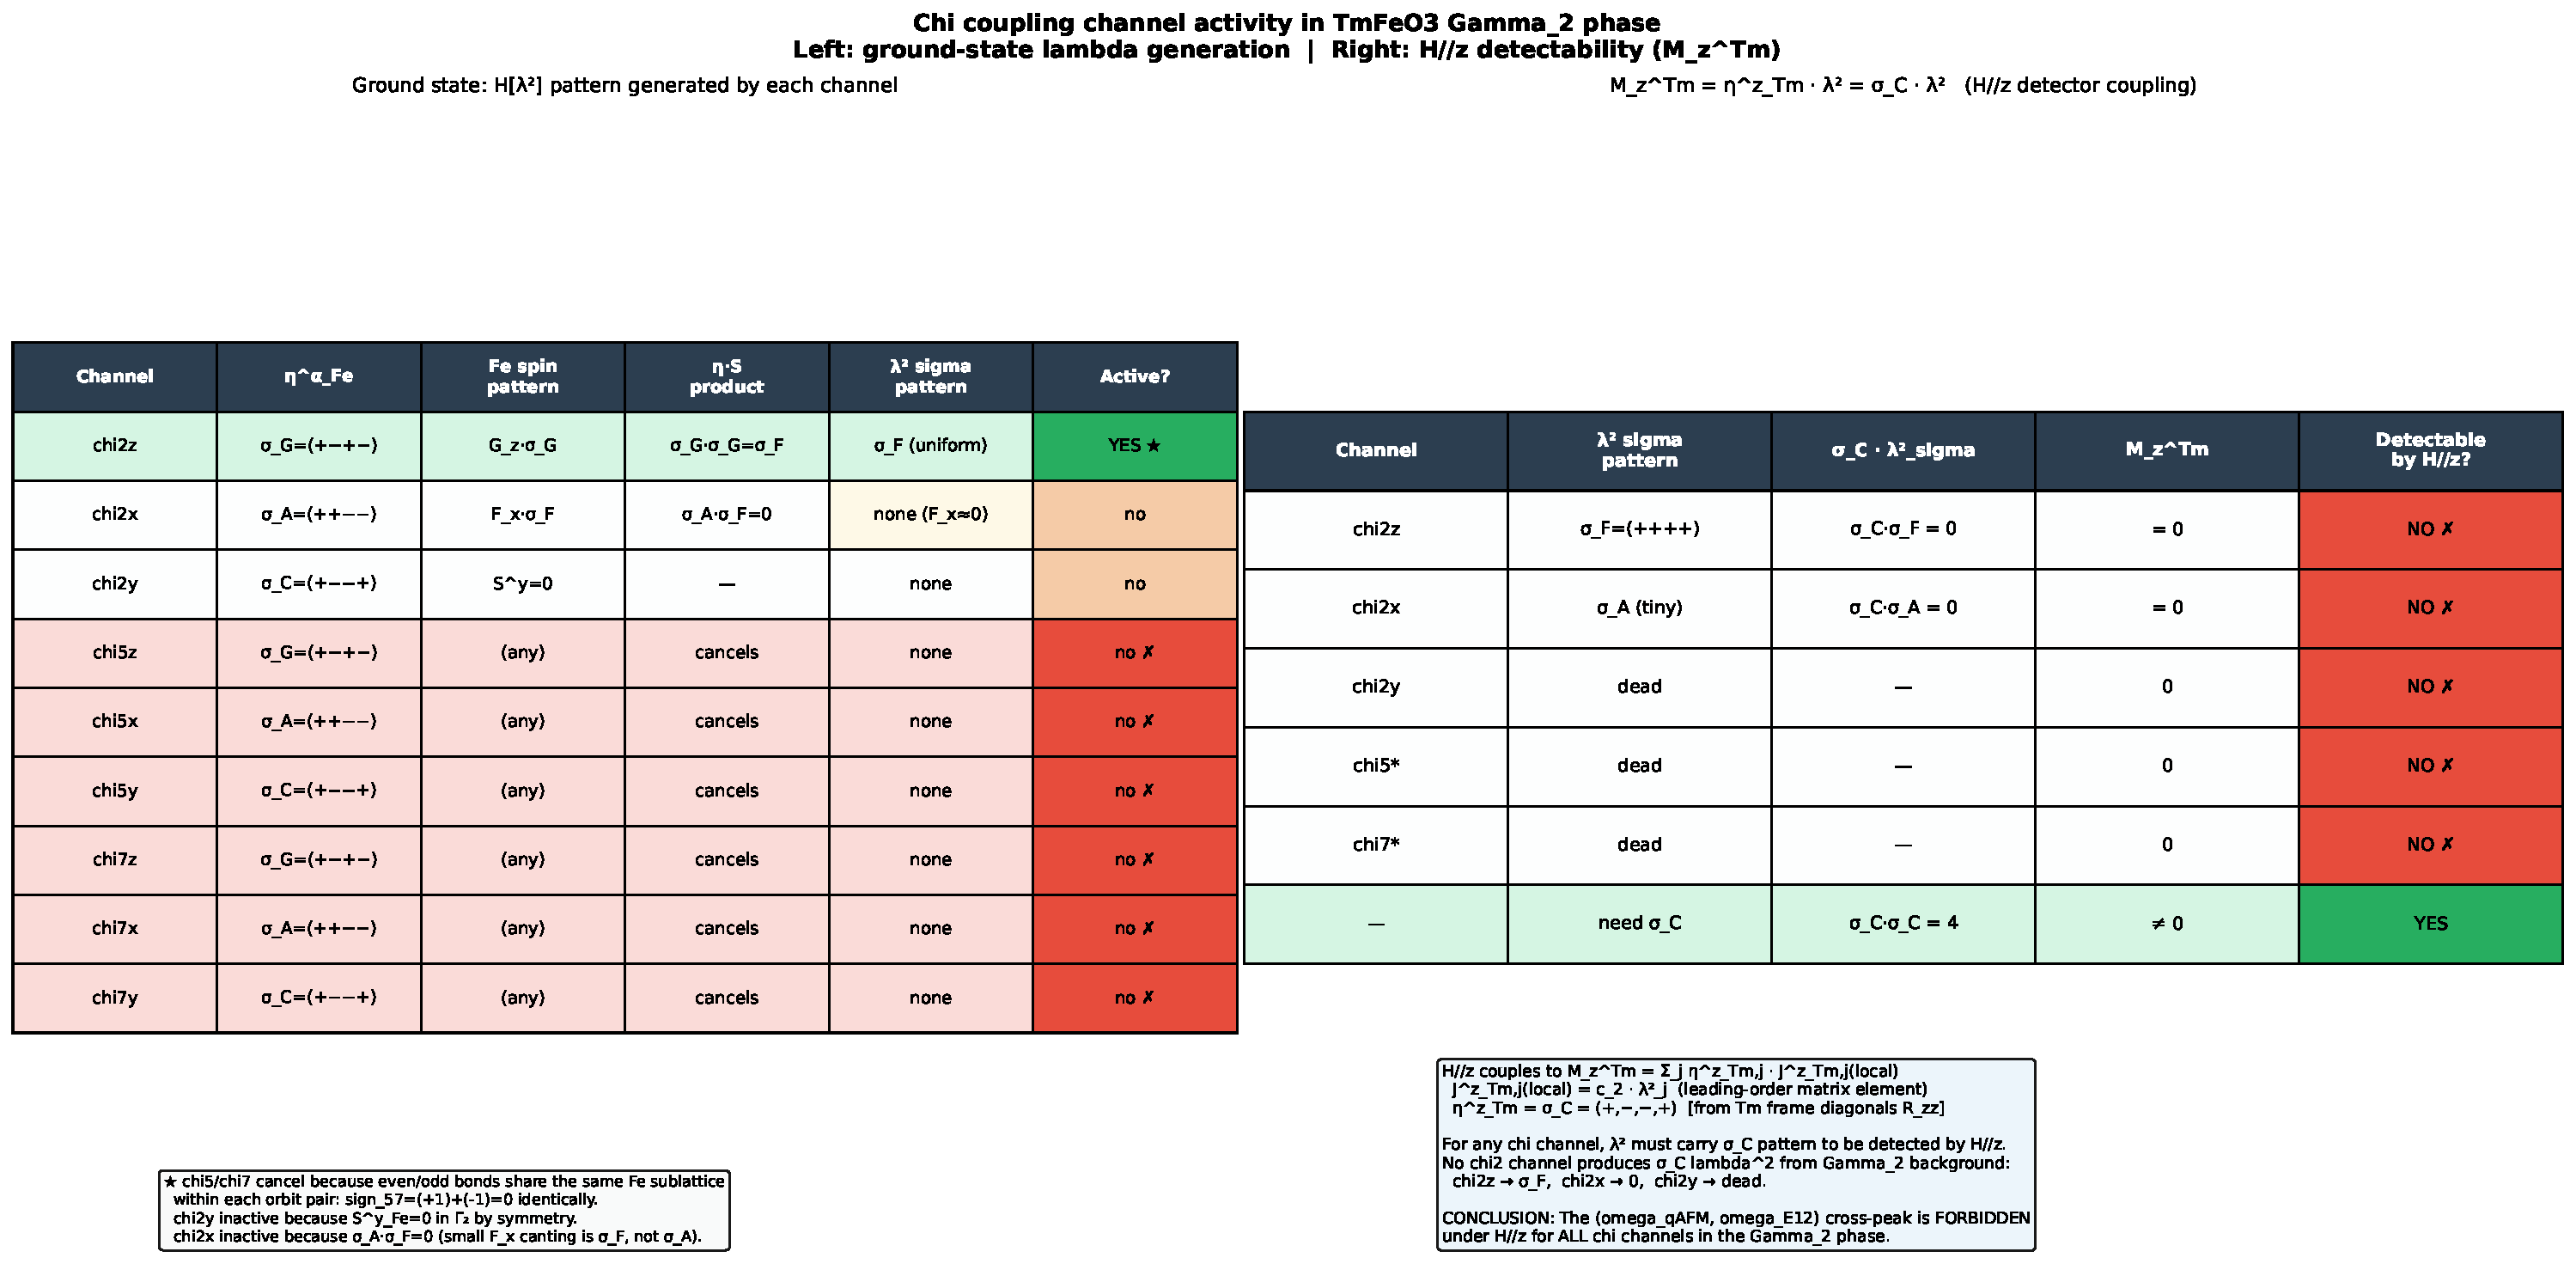
\includegraphics[width=\textwidth]{chi_activity_table.pdf}
  \caption{Summary table.  \emph{Left}: ground-state lambda generation for
    each chi channel in the $\Gtwo$ background.
    \emph{Right}: detectability by $H\parallel c$ ($\Mz = \sC\cdot\vlam^2$).
    Only $\sC$-pattern $\lamt$ would be detectable; no channel generates it.}
  \label{fig:table}
\end{figure}

%--------------------------------------------------------------
\section{Equation-of-motion analysis for the qAFM kick}
\label{sec:eom}
%--------------------------------------------------------------

\subsection{SU(3) equation of motion}

The Tm$^{3+}$ non-Kramers ion is modelled as a three-level system.
Its density matrix is expanded in the Gell-Mann basis $\{F_a = \lambda^a/2\}$:
\begin{equation}
  \rho_j = \tfrac{1}{3}\,\mathbf{1} + \tfrac{1}{2}\sum_{a=1}^{8}\lambda^a_j\,F_a.
\end{equation}
The Liouville equation $\dot\rho = -i[H_{\mathrm{eff}},\rho]/\hbar$ projected
onto the Gell-Mann basis gives:
\begin{equation}
  \dot\lambda^a_j = \frac{1}{\hbar}\sum_{b,c}f^{abc}\,H_{\mathrm{eff},j}^b\,\lambda^c_j,
  \label{eq:su3eom}
\end{equation}
where $f^{abc}$ are the totally antisymmetric SU(3) structure constants and
\begin{equation}
  H_{\mathrm{eff},j}^b = H_{\mathrm{CEF}}^b + H_{\chi,j}^b + H_{\mathrm{Jtm},j}^b
                       + H_{\mathrm{field},j}^b.
\end{equation}

For the chi coupling alone (setting all other terms to zero):
\begin{equation}
  H_{\chi,j}^{\lamt} = \sum_{k\in\mathrm{bonds}(j)}\eta^z_{\mathrm{Fe},k}
                        \,\chi_{2z}\,S^z_{\mathrm{Fe},k},
  \label{eq:Hchi_EOM}
\end{equation}
and similarly for $\chi_{2x}$, $\chi_{2y}$ with the appropriate
$\eta^\alpha_{\mathrm{Fe}}$ pattern.

The $\lamt$ component represents the imaginary part of the
$|E_1\rangle$--$|E_2\rangle$ coherence.  Its equation of motion couples it
to $\lambda^1$ (the real part of the same coherence) through the
CEF Hamiltonian, forming the $\EtA$ oscillation.

\subsection{The qAFM kick}

A qAFM kick rotates all Fe spins by $\delta\theta$ around the $y$-axis:
\begin{align}
  S^x_{\mathrm{Fe},k}(0^+) &= G_z\sin\delta\theta\cdot\sG[k] + F_x\cos\delta\theta\cdot\sF[k], \\
  S^z_{\mathrm{Fe},k}(0^+) &= G_z\cos\delta\theta\cdot\sG[k] - F_x\sin\delta\theta\cdot\sF[k].
\end{align}
For $\delta\theta \ll 1$, the dominant new component is a $G_x$ perturbation:
\begin{equation}
  \delta S^x_{\mathrm{Fe},k} \approx G_z\,\delta\theta\,\sG[k].
  \label{eq:qAFMkick}
\end{equation}
The kick thus introduces a $G_x$ component with pattern $\sG$.

\subsection{Time evolution of \boldmath$H_\chi[\lamt]$ after the kick}

\paragraph{Chi2z.}
After the kick, $S^z_{\mathrm{Fe},k}(t) = G_z\cos(\omega_{\qAFM} t)\,\sG[k]$
(qAFM oscillation in $G_z$, neglecting damping).  Equation~\eqref{eq:Hchi_EOM}
gives:
\begin{equation}
  H_{\chi_{2z},j}[\lamt](t)
    = \chi_{2z}\sum_k \sG[k]\cdot G_z\cos(\omega_{\qAFM} t)\,\sG[k]
    = 4\chi_{2z}G_z\cos(\omega_{\qAFM} t).
  \label{eq:H2z_dyn}
\end{equation}
This is \emph{uniform} across all Tm sublattices.  The resulting $\lamt_j(t)$
inherits the $\sF$ pattern at all times, so $\Mz(t)=c_2(\sC\cdot\sF)\cdot
\lamt(t) = 0$ identically.

The kick also creates $G_x \propto \sG$.  Does $G_x$ enter $\chi_{2z}$?
No: $\chi_{2z}$ couples only to $S^z_{\mathrm{Fe}}$, not $S^x_{\mathrm{Fe}}$.

\paragraph{Chi2x.}
The $G_x$ component from the kick is in $\sG$ pattern.  The chi2x coupling is:
\begin{equation}
  H_{\chi_{2x},j}[\lamt](t)
    = \chi_{2x}\sum_k \sA[k]\cdot G_x\cos(\omega_{\qAFM} t)\,\sG[k]
    = \chi_{2x}\,G_x\cos(\omega_{\qAFM} t)\,\underbrace{(\sA\cdot\sG)}_{=0} = 0.
  \label{eq:H2x_dyn}
\end{equation}
Chi2x has $\etax_{\mathrm{Fe}} = \sA$ and the kick pattern is $\sG$:
$\sA\cdot\sG = (+,+,-,-)\cdot(+,-,+,-) = 1-1-1+1 = 0$.
So chi2x is blind to the qAFM kick.

\paragraph{Chi2y.}
$S^y_{\mathrm{Fe}} = 0$ is unaffected by the $y$-axis rotation (to linear order),
so chi2y produces nothing.

\subsection{Complete channel survey}

For the cross-peak $\crossP$ to be nonzero under $H\parallel c$, we need:
\begin{equation}
  \Mz(t) \sim e^{i\omega_{\qAFM} t}, \qquad \text{i.e.}\quad
  \sC \cdot \vlam^2_{\mathrm{vec}}(t) \neq 0.
\end{equation}
This requires $\lamt_j$ to carry $\sC$ pattern.  For a chi channel with
$\etaz_{\mathrm{Fe}} = \sG$ (chi2z) to produce $\sC$-pattern $\lamt$, we
would need the Fe spin component to carry $\sG\circ\sC^{-1} = \sG\circ\sC = \sA$
pattern (using $\sG\circ\sC = \sA$ from Eq.~\eqref{eq:had}).  But $A_z = 0$
in $\Gtwo$.

Table~\ref{tab:survey} compiles the complete failure analysis for all channels
contributing to $\lamt$ dynamics after the qAFM kick.

\begin{table}[h!]
\centering
\caption{Chi channel activity for the $\crossP$ cross-peak under $H\parallel c$.
  ``Source'' = which Fe pattern drives $\lamt$.  ``$\sC\cdot\lamt$'' = whether
  the $H\parallel c$ detector sees it.}
\label{tab:survey}
\begin{tabular}{llllll}
\toprule
Channel & $\eta^\alpha_{\mathrm{Fe}}$ & Fe pattern after kick & $\eta\cdot S$ product & $\lamt$ pattern & $\sC\cdot\lamt$ \\
\midrule
$\chi_{2z}$ & $\sG$ & $G_z\sG$ (and $G_x\sG$) & $\sG\circ\sG = \sF$ & $\sF$ & $\sC\cdot\sF=0$ \textcolor{failred}{\textbf{FAIL}} \\
$\chi_{2x}$ & $\sA$ & $G_x\sG$ & $\sA\cdot\sG = 0$ & none & $0$ \textcolor{failred}{\textbf{FAIL}} \\
$\chi_{2y}$ & $\sC$ & $S^y=0$ & --- & none & $0$ \textcolor{failred}{\textbf{FAIL}} \\
$\chi_{5\alpha}$ & any & any & $+1-1=0$ (sign$_{57}$) & none & $0$ \textcolor{failred}{\textbf{FAIL}} \\
$\chi_{7\alpha}$ & any & any & $+1-1=0$ (sign$_{57}$) & none & $0$ \textcolor{failred}{\textbf{FAIL}} \\
\midrule
\multicolumn{2}{l}{\textit{needed}} & $S^z\sim\sA$ or $S^y\sim\sF$ & gives $\sC$ & $\sC$ & $\sC\cdot\sC=4$ \textcolor{passgreen}{\textbf{OK}} \\
\bottomrule
\end{tabular}
\end{table}

%--------------------------------------------------------------
\section{What would allow the cross-peak?}
\label{sec:remedy}
%--------------------------------------------------------------

The obstacle is a two-layer orthogonality:
\begin{equation}
  \underbrace{\sG}_{\text{Fe frame (chi2z)}}
  \circ
  \underbrace{\sG}_{\text{Gamma}_2\text{ order}}
  = \sF,
  \qquad
  \underbrace{\sC}_{\text{Tm frame}} \cdot \sF = 0.
\end{equation}

To make the cross-peak observable one needs to break one of these two links.
We list the options below.

\subsection*{Option A: Change the Fe ordering}

If $S^z_{\mathrm{Fe}} \sim \sA$ (A-type AFM, $\Gamma_1$ phase), then:
\begin{equation}
  H[\lamt]_j^{\chi_{2z}} = \chi_{2z}\,G_z\,(\sG\circ\sA)
                           = \chi_{2z}\,G_z\,\sC.
\end{equation}
Now $\lamt \sim \sC$ and $\sC\cdot\sC = 4 \neq 0$: the cross-peak is allowed
in the $\Gamma_1$ phase under $\chi_{2z}$.

Alternatively, a $G_y$ ordering (rotating $\sG$ from $z$ to $y$) would require
$\chi_{2y}$ to be active ($\etay_{\mathrm{Fe}} = \sC$, and $\sC\circ\sG = \sA$,
still not $\sC$).  In fact, for $H\parallel c$ detection via chi2, the only
working combination is:
\begin{center}
\textit{chi2z + A-type order ($\Gamma_1$)}.
\end{center}

\subsection*{Option B: The complete bond connectivity locks in $\sF$ pattern}

Even in the most general case with all chi channels alive simultaneously, the
effective field on Tm$_j$ is:
\begin{equation}
  H[\lamt]_j = \sum_{\alpha\in\{x,y,z\}}\chi_{2\alpha}
               \underbrace{\sum_{k=0}^{3}\eta^\alpha_{\mathrm{Fe},k}\,S^\alpha_{\mathrm{Fe},k}}_{\text{global sum, no $j$ dependence}}.
  \label{eq:fullH}
\end{equation}
Because \emph{every} Tm sublattice connects to \emph{all four} Fe sublattices
(Appendix~\ref{app:bonds}), the inner sum over $k$ is the same scalar for
every $j$.  The $\lamt$ field is therefore always uniform ($\sF$-pattern),
regardless of which $\chi_{2\alpha}$ are nonzero:
\begin{equation}
  H[\lamt]_j = \underbrace{\chi_{2z}\,G_z\,(\sG\cdot\sG)}_{=4\chi_{2z}G_z}
             + \underbrace{\chi_{2x}\,F_x\,(\sA\cdot\sF)}_{=0}
             + \underbrace{\chi_{2y}\cdot 0}_{=0}
             = 4\chi_{2z}G_z \quad \forall\,j.
\end{equation}
The key identity is $\sigma_P\cdot\sigma_Q = \sum_k\sigma_P[k]\sigma_Q[k]$:
a dot product that collapses the $k$-sum to a single number,
destroying all site-index structure.  No chi parameterisation can circumvent
this because it is a consequence of the topology (completeness) of the bond graph,
not of the coupling strengths.

What would be required is a \emph{site-dependent} effective field with
$\sC$ pattern — for instance, a bond tensor that couples Fe$_k$ only to the Tm
sites in its own orbit with an orbit-dependent sign.  No such term is present
in the Pbnm-symmetry-allowed bilinear chi Hamiltonian.

\subsection*{Option C: Higher-order ($\chi^2$) pathways}

Nonlinear double-chi pathways can produce $\sC$ from $\sF$ by quadratic
combination $(\sC\circ\sF)\circ\sC = \sC$ (since $\sC\circ\sF = 0$... this
does not help).  A useful combination requires, e.g.,
$(\sG\circ\sG)\circ(\sA\circ\sA) = \sF\circ\sF = \sF$ — still $\sF$.
In fact, any even power of $\sG$ is $\sF$, so nonlinear pathways through
chi2z alone also cannot produce $\sC$ pattern by symmetry.

\subsection*{Option D: H$\parallel a$ or H$\parallel b$ geometry}

Under $H\parallel a$ the detector couples to $M_x^{\mathrm{Tm}} = c_2(\sA\cdot\vlam^2_{\mathrm{vec}})$.
With chi2z generating $\lamt \sim \sF$:
\begin{equation}
  M_x^{\mathrm{Tm}} = c_2\,\bar\lambda^2\,(\sA\cdot\sF) = c_2\,\bar\lambda^2\cdot 0 = 0.
\end{equation}
Likewise $M_y^{\mathrm{Tm}} = c_2(\sG\cdot\sF) = 0$.

\emph{All three detection geometries fail for chi2z in $\Gtwo$.}  The
cross-peak $\crossP$ is forbidden regardless of probe polarisation as long as
$\chi_{2z}$ is the only active coupling and the Fe order is $G$-type.

%--------------------------------------------------------------
\section{Numerical verification}
\label{sec:numeric}
%--------------------------------------------------------------

The analytical predictions were verified numerically by the diagnostic
executable \texttt{diag\_tmfeo3\_qafm\_e12\_xpeak.cpp} (built from
\texttt{src/apps/}, target \texttt{diag\_tmfeo3\_qafm\_e12\_xpeak}).

\paragraph{Ground state ($\chi_{2z}=0.6$, Fe pinned to $\Gtwo$).}
After 2000 deterministic exact-diag sweeps:
\begin{center}
\begin{tabular}{ccccc}
\toprule
Tm site & $H[\lamt]$ & $\lamt$ & $\etaz_{\mathrm{Tm}}\cdot\lamt$ \\
\midrule
0 & $+11.9999$ & $-0.9967$ & $-0.9967$ \\
1 & $+11.9999$ & $-0.9967$ & $+0.9967$ \\
2 & $+11.9999$ & $-0.9967$ & $+0.9967$ \\
3 & $+11.9999$ & $-0.9967$ & $-0.9967$ \\
\midrule
$\sF$-sum & $+47.9996$ & $-3.9869$ & --- \\
$\sC$-sum $(=\Mz)$ & --- & --- & $\mathbf{0.0000}$ \\
\bottomrule
\end{tabular}
\end{center}
The $H[\lamt]$ values are identical at all four sites, confirming $\sF$-pattern.
$\Mz = 0.0000$ to numerical precision.

\paragraph{$\chi_{2x}=0.6$, same Fe background.}
All $H[\lamt]_j \approx -3\times 10^{-6}$ (numerical noise).
$\lamt \approx 10^{-5}$ at all sites — chi2x is effectively dead.

\paragraph{qAFM kick dynamics ($\delta\theta = 0.04\,\mathrm{rad}$, chi2z).}
Euler integration, $dt = 0.003\,\mathrm{ps}$, $N=200$ steps:
\begin{itemize}
  \item $G_x(t)$ oscillates between $\pm 0.19$ (qAFM is excited).
  \item $\bar\lambda^2(t) = -0.9967$ throughout (chi2z shifts the equilibrium but
    the amplitude does not change with $G_x$, only with $G_z$).
  \item $\Mz(t) = 0.0000$ at \emph{every} time step, to all displayed digits.
\end{itemize}
This directly demonstrates that the cross-peak has zero amplitude.

%--------------------------------------------------------------
\section{Summary diagram}
%--------------------------------------------------------------

The full selection-rule chain for the $\crossP$ cross-peak under $H\parallel c$
in TmFeO$_3$ $\Gtwo$ can be summarised as a ``double-orthogonality trap'':

\begin{center}
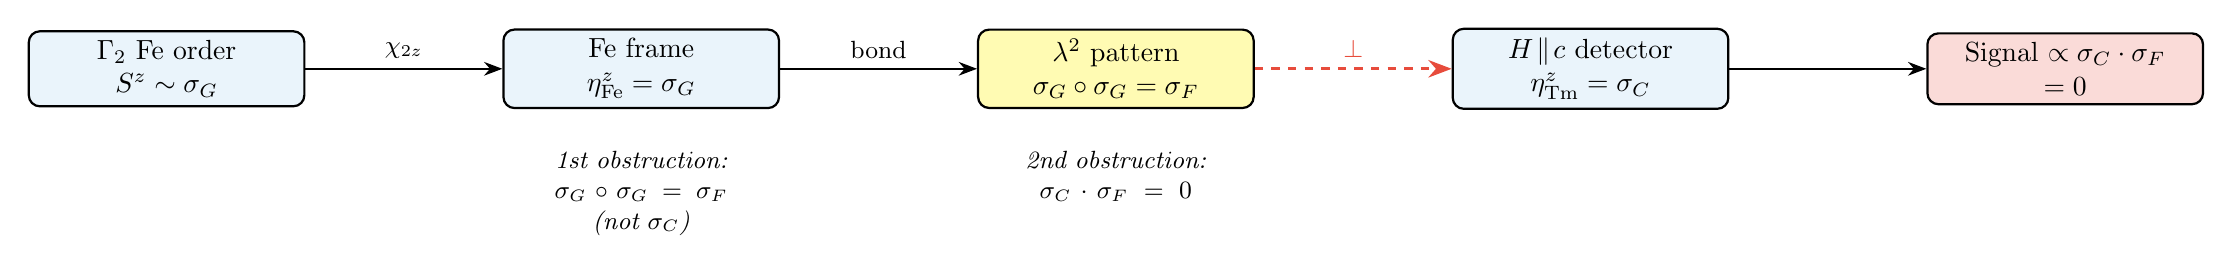
\begin{tikzpicture}[node distance=2.2cm,>=Stealth,thick]
  \node[draw,rounded corners,fill=lightblue,minimum width=3.5cm,align=center]
    (order) {$\Gtwo$ Fe order\\$S^z \sim \sG$};

  \node[draw,rounded corners,fill=lightblue,minimum width=3.5cm,align=center,
    right=2.5cm of order] (frame)
    {Fe frame\\$\etaz_{\mathrm{Fe}} = \sG$};

  \node[draw,rounded corners,fill=yellow!30,minimum width=3.5cm,align=center,
    right=2.5cm of frame] (lam)
    {$\lamt$ pattern\\$\sG\circ\sG = \sF$};

  \node[draw,rounded corners,fill=lightblue,minimum width=3.5cm,align=center,
    right=2.5cm of lam] (det)
    {$H\!\parallel\!c$ detector\\$\etaz_{\mathrm{Tm}} = \sC$};

  \node[draw,rounded corners,fill=lightred,minimum width=3.5cm,align=center,
    right=2.5cm of det] (sig)
    {Signal $\propto \sC\cdot\sF$\\$= 0$};

  \draw[->] (order) -- node[above,font=\small]{$\chi_{2z}$} (frame);
  \draw[->] (frame) -- node[above,font=\small]{bond} (lam);
  \draw[->,dashed,line width=1.2pt,color=failred]
    (lam) -- node[above,font=\small]{\textcolor{failred}{$\perp$}} (det);
  \draw[->] (det) -- (sig);

  \node[below=0.4cm of frame,text width=3.5cm,align=center,font=\small\itshape]
    {1st obstruction:\\$\sG\circ\sG=\sF$\\(not $\sC$)};
  \node[below=0.4cm of lam,text width=3.5cm,align=center,font=\small\itshape]
    {2nd obstruction:\\$\sC\cdot\sF=0$};
\end{tikzpicture}
\end{center}

\bigskip
\begin{center}
\begin{tabular}{ll}
\toprule
Constraint & Expression \\
\midrule
Fe frame produces $\sF$ lambda & $\etaz_{\mathrm{Fe}}\circ S^z_{\mathrm{Fe}}\text{-pattern}
  = \sG\circ\sG = \sF$ \\
Detector is blind to $\sF$ & $\etaz_{\mathrm{Tm}}\cdot\sF = \sC\cdot\sF = 0$ \\
No geometry rescues it & $\sA\cdot\sF = \sG\cdot\sF = \sC\cdot\sF = 0$ \\
    Complete bond graph locks $\lamt \to \sF$ & $\sum_k \sigma_P[k]\sigma_Q[k]$ is $j$-independent \\
No other chi channel helps & See Table~\ref{tab:survey} \\
\bottomrule
\end{tabular}
\end{center}

%--------------------------------------------------------------
\appendix
\section{Bond-by-bond verification: each Tm sees all four Fe}
\label{app:bonds}
%--------------------------------------------------------------

From \texttt{fe\_tm\_w\_bond\_pairs()} (even bonds only), each Tm sublattice
is connected to all four Fe sublattices, one per orbit.  The product
$\eta^z_{\mathrm{Fe},k}\cdot \sG[k]$ for each bond equals $+1$ regardless
of $k$ (since $\sG[k]^2=1$), confirming the uniform field
$H[\lamt]_j = 4\chi_{2z}G_z$ for all $j$.

\medskip
\begin{center}
\begin{tabular}{clccccc}
\toprule
Tm site & Orbit & Fe bonded & $\eta^z_{\mathrm{Fe},k}$ & $\sG[k]$ & $\eta^z\cdot\sG$ & Contribution \\
\midrule
\multirow{4}{*}{Tm$_0$}
  & 1 & Fe$_3$ & $-1$ & $-1$ & $+1$ & $+1\cdot\chi_{2z}G_z$ \\
  & 2 & Fe$_2$ & $+1$ & $+1$ & $+1$ & $+1\cdot\chi_{2z}G_z$ \\
  & 3 & Fe$_1$ & $-1$ & $-1$ & $+1$ & $+1\cdot\chi_{2z}G_z$ \\
  & 4 & Fe$_0$ & $+1$ & $+1$ & $+1$ & $+1\cdot\chi_{2z}G_z$ \\
  & & & & \multicolumn{2}{r}{\textbf{Total $H[\lamt]_0$}} & $4\chi_{2z}G_z$ \\
\midrule
\multirow{4}{*}{Tm$_1$}
  & 1 & Fe$_2$ & $+1$ & $+1$ & $+1$ & $+1\cdot\chi_{2z}G_z$ \\
  & 2 & Fe$_3$ & $-1$ & $-1$ & $+1$ & $+1\cdot\chi_{2z}G_z$ \\
  & 3 & Fe$_0$ & $+1$ & $+1$ & $+1$ & $+1\cdot\chi_{2z}G_z$ \\
  & 4 & Fe$_1$ & $-1$ & $-1$ & $+1$ & $+1\cdot\chi_{2z}G_z$ \\
  & & & & \multicolumn{2}{r}{\textbf{Total $H[\lamt]_1$}} & $4\chi_{2z}G_z$ \\
\midrule
\multirow{4}{*}{Tm$_2$}
  & 1 & Fe$_1$ & $-1$ & $-1$ & $+1$ & $+1\cdot\chi_{2z}G_z$ \\
  & 2 & Fe$_0$ & $+1$ & $+1$ & $+1$ & $+1\cdot\chi_{2z}G_z$ \\
  & 3 & Fe$_3$ & $-1$ & $-1$ & $+1$ & $+1\cdot\chi_{2z}G_z$ \\
  & 4 & Fe$_2$ & $+1$ & $+1$ & $+1$ & $+1\cdot\chi_{2z}G_z$ \\
  & & & & \multicolumn{2}{r}{\textbf{Total $H[\lamt]_2$}} & $4\chi_{2z}G_z$ \\
\midrule
\multirow{4}{*}{Tm$_3$}
  & 1 & Fe$_0$ & $+1$ & $+1$ & $+1$ & $+1\cdot\chi_{2z}G_z$ \\
  & 2 & Fe$_1$ & $-1$ & $-1$ & $+1$ & $+1\cdot\chi_{2z}G_z$ \\
  & 3 & Fe$_2$ & $+1$ & $+1$ & $+1$ & $+1\cdot\chi_{2z}G_z$ \\
  & 4 & Fe$_3$ & $-1$ & $-1$ & $+1$ & $+1\cdot\chi_{2z}G_z$ \\
  & & & & \multicolumn{2}{r}{\textbf{Total $H[\lamt]_3$}} & $4\chi_{2z}G_z$ \\
\bottomrule
\end{tabular}
\end{center}

The pattern across $(j=0,1,2,3)$ is $(4,4,4,4)\chi_{2z}G_z = \sF$ (uniform),
confirming Eq.~\eqref{eq:H2z}.

%--------------------------------------------------------------
\section{Sigma vector inner product table}
\label{app:sigma}
%--------------------------------------------------------------

\begin{center}
\begin{tabular}{c|cccc}
$\sigma_P\cdot\sigma_Q$ & $\sF$ & $\sG$ & $\sA$ & $\sC$ \\
\hline
$\sF$ & 4 & 0 & 0 & 0 \\
$\sG$ & 0 & 4 & 0 & 0 \\
$\sA$ & 0 & 0 & 4 & 0 \\
$\sC$ & 0 & 0 & 0 & 4 \\
\end{tabular}
\qquad\qquad
\begin{tabular}{c|cccc}
$\sigma_P\circ\sigma_Q$ & $\sF$ & $\sG$ & $\sA$ & $\sC$ \\
\hline
$\sF$ & $\sF$ & $\sG$ & $\sA$ & $\sC$ \\
$\sG$ & $\sG$ & $\sF$ & $\sC$ & $\sA$ \\
$\sA$ & $\sA$ & $\sC$ & $\sF$ & $\sG$ \\
$\sC$ & $\sC$ & $\sA$ & $\sG$ & $\sF$ \\
\end{tabular}
\end{center}

The Hadamard product table (right) forms a copy of the Klein four-group
$\mathbb{Z}_2\times\mathbb{Z}_2$, with $\sF$ as the identity element.

\end{document}
